\documentclass[12pt,twoside,titlepage]{ingenius}
\usepackage[figuresright]{rotating}
\usepackage{pgfplots} 
\pgfplotsset{compat=1.7}
\usepackage{adjustbox}
\usepackage{units}
\usepackage{dblfloatfix}
\usepackage{amssymb}
\usepackage{caption}
\usepackage{subcaption}
\usepackage{bm}
\usepackage{textcomp}
\usepackage{pifont}
\usepackage{cite}
\usepackage{xcolor,colortbl}
\usepackage{amsmath}
\usepackage{upgreek}
\usepackage{graphicx}
\usepackage{tikz}%flujogramas
\usepackage{pifont}
\usetikzlibrary{shapes,arrows}
\usepackage{textcomp}
\usepackage{multirow}
\usepackage{float}
\usepackage{soul}
\usepackage{rotating}
\usepackage{hyperref}
\usepackage{booktabs}
\usepackage{algorithmic}
\usepackage[ruled,vlined,algo2e]{algorithm2e}
\usepackage{algorithm}
%\usepackage{fancyhdr}
%\pagestyle{fancy}
\makeatletter
\renewcommand*{\ALG@name}{Algoritmo}
\makeatother
\graphicspath{{figures/}}
%===========================================
%========
\usepackage{tikz,xcolor,hyperref}
% Make Orcid icon
\definecolor{lime}{HTML}{A6CE39}
\DeclareRobustCommand{\orcidicon}{%
	
\begin{tikzpicture}
	\draw[lime, fill=lime] (0,0) 
	circle [radius=0.16] 
	node[white] {{\fontfamily{qag}\selectfont \tiny ID}};
	\draw[white, fill=white] (-0.0625,0.095) 
	circle [radius=0.007];
	\end{tikzpicture}
	\hspace{-2mm}
}
\foreach \x in {A, ..., Z}{%
	\expandafter\xdef\csname orcid\x\endcsname{\noexpand\href{https://orcid.org/\csname orcidauthor\x\endcsname}{\noexpand\orcidicon}}
}
%========================================================
\titulo{Inteligencia artificial y accesibilidad educativa en lenguas de bajos recursos: una revisión sistemática de usos, desafíos y oportunidades}
\tituloa{A Systematic Review of Artificial Intelligence for Improving Educational Accessibility in Low-Resource Languages: Uses, Challenges, and Opportunities}
%========================================================
\newcommand{\orcidauthorA}{0009-0006-0590-6700}
\autores{Lorena Kim Negrillo $^{1}$,\orcidA{}}
\adscripcionautor{%
$^{1}$ En esta sección escriba la adscripción institucional actual en el siguiente orden: Dependencia a la que pertenece en su institución, Institución a la que pertenece,  país.\\
$^{2}$Laboratorio de Investigación en Sistemas Informáticos e Inteligencia Artificial, Universidad Politécnica de Valencia - España.\\
$^{3}$ Autor 3, Dependencia, Institución, Ciudad, País, e-mail: correoelectrónico@autorparacorrespondencia}

%%Datos para referencias
\newcommand{\apellido}{Kim Negrillo}% Apellido o apellidos para referencia 
\newcommand{\titu}{Inteligencia artificial y accesibilidad educativa en lenguas de bajos recursos: una revisión sistemática de usos, desafíos y oportunidades}%titulo a la ref\erencia
\newcommand{\tipo}{Art\'iculo Cient\'if{}ico / Scientif{}ic Paper} 
%tipo de documento Punto de vista/Point of view,  Art\'iculo Cient\'if{}ico / Scientif{}ic Paper, Rese\~na bibliogr\'afica/Review
%========================================================
%%Datos para propiedades del pdf no requiere ser llenado
\newcommand{\autor}{}%autor para propiedades del pdf
\newcommand{\pc}{}%palabras clave para propiedades del pdf
\newcommand{\kw}{}%keywords para propiedades del pdf
\usepackage{xcolor}
\usepackage{color}
\input{configuracion_paquetes}
%\input{config_c}
\usepackage{listings}%% lista de códigos
	\lstset{ 
		linewidth=0.5\textwidth,
		frame=tb,	
		%framerule=0.5pt,
		aboveskip=0.5cm,%Distancia Texto al codigo
		%framextopmargin=3pt,%Distancia Primera Linea-Borde Superior
		framexbottommargin=3pt,%Distancia Ultima Linea-Borde Inferior
		%framexleftmargin=0.4cm,%Distancia Borde Izquierdo Codigo-Borde Izquierdo Pagina
		framesep=0pt,
		rulesep=.8pt,%Espesor linea junto a los numeros
		backgroundcolor=\color{gray!10},
                     numbersep=5pt,
                     xleftmargin=3pt,
                     xrightmargin=8.5pt,
                     framextopmargin=10pt,
		rulesepcolor=\color{black},
		stringstyle=\ttfamily,
		floatplacement=htb,
		boxpos={c},
		breaklines=true,
		breakatwhitespace=true,
		showstringspaces = false,
		basicstyle=\small\ttfamily,
		commentstyle=\color{gray!45},
		keywordstyle=\bfseries,
		%linewidth=0.8\textwidth,
		title=\lstname,
		%numbers=right,%Posicion de los Numeros left=izquierda; right=derecha
		%numbersep=15pt, %separacion de numero 1,2,3,4 hacia el frame
		numberstyle=\tiny,
		numberfirstline = false,
		breaklines=true,
		}
	\lstnewenvironment{listing}[1][]
		{\lstset{#1}\pagebreak[0]}{\pagebreak[0]}
		\lstdefinestyle{consola}
		{basicstyle=\scriptsize\bf\ttfamily,
		 backgroundcolor=\color{gray75},
		}
	\lstdefinestyle{C}
		{language=C,
}

\newenvironment{tabla}
  {\par\bigskip\noindent\minipage{\linewidth}}
  {\endminipage\par\bigskip}

\newenvironment{figura}
  {\par\bigskip\noindent\minipage{\linewidth}}
  {\endminipage\par\bigskip}

\newenvironment{pseudo}
  {\par\noindent\minipage{\linewidth}}
  {\endminipage\par\bigskip}
%========================================================
\begin{document}
\renewcommand{\lstlistingname}{Algorithm}
\setcounter{page}{1}
\renewcommand{\refname}{Referencias}
\renewcommand{\figurename}{Figura}
\renewcommand{\tablename}{Tabla}
\frenchspacing

\begin{tikzpicture}[overlay]
  \node at (138.5mm,12.2mm){
\includegraphics[scale=0.35]{figures/logoingenius.pdf}};
 \node at (138mm,2mm){\textsf{\scriptsize pISSN: 1390-650X / eISSN: 1390-860X}};
   \node at (79mm,10mm){
\includegraphics[scale=0.6]{figures/creativec.pdf}};
\end{tikzpicture}

\input{silabeo}
\membrete
\input{configuracion_portada}

%\begin{textblock}{12.4}(0,10)
\begin{textblock}{12.4}(0,10)%Modificar Editor Ingenius cuando se inserte Creative Commons
\adscripcion
\end{textblock}
%========================================================
\begin{table}[htb]
\begin{tabular}{p{8cm}p{8cm}}
{\Large \bfseries Resumen} &{\Large \bfseries Abstract} \\ \\
Bajo el marco de trabajo PRISMA, se realizó una revisión sistemática de la literatura en la base de datos Scopus, donde se analizaron 27 artículos publicados entre los años 2022 y 2026. Los resultados revelaron que si bien modelos multilingües no se desempeñan correctamente en lenguas de bajos recursos, por ejemplo, el modelo \textit{Cross-Lingual Language Modeling-Roberta}(XLM-R) en un escenario \textit{zero-shot} sobre 10 lenguas indígenas obtuvo una presición promedio de 38.48\%, existen enfoques que permiten obtener resultados más favorables, como el uso de meta-aprendizaje (MAML), implementación de arquitecturas hibridas, inyección de conocimiento lingüistico y un enfoque participativo con la población de estudio. Aún existen limitaciones que son necesarias de abarcar en futuras investigaciones, como la escacez de datos y falta de recursos computacionales, la necesidad de un enfoque participativo y métricas especializadas para lenguas de bajos recursos lingüisticos, por tal motivo se sugiere que los investigadores adopten enfoques participativos y prioricen las necesidades con los hablantes de las lenguas estudiadas.

&Under the PRISMA methodology, a systematic literature review was conducted using the Scopus database, in which 27 articles published between 2022 and 2026 were analyzed. The results revealed that, although multilingual models do not perform adequately in low-resource languages—for example, the \textit{Cross-Lingual Language Modeling-Roberta} (XLM-R) model achieved an average accuracy of 38.48\% in a \textit{zero-shot} scenario across 10 Indigenous languages—there are approaches that make it possible to obtain more favorable results, such as the use of meta-learning (MAML), the implementation of hybrid architectures, the injection of linguistic knowledge, and a participatory approach involving the study population. There are still limitations that need to be addressed in future research, such as data scarcity and the lack of computational resources, the need for a participatory approach, and specialized metrics for low-resource languages. Therefore, it is suggested that researchers adopt participatory approaches and prioritize needs together with the speakers of the languages being studied.
……………..
\\[-0.3cm]
\palabrasclave{Aprendizaje, aprendizaje personalizado, enseñanza, equidad educativa, Inteligencia Artificial, lenguas con pocos recursos, pedagogía, procesamiento del lenguaje natural.}&\keywords{Artificial Intelligence, educational equity, learning, low-resource languages, natural language processing, pedagogy, personalized learning, teaching.}  \\
\end{tabular}
\end{table}

\newpage

\begin{multicols}{2}
%========================================================
\section{Introducción}
\vspace{-0.15cm}

La Organización de las Naciones Unidas para la Educación, la Ciencia y la Cultura (UNESCO) señala que el 40\% de la población mundial no tiene acceso a
educación en una lengua que hable y comprenda con fluidez. Si bien este problema afecta a la población en general, su impacto en las personas cuyas lenguas
maternas corresponden a lenguas de bajos recursos es mucho más drástico  \cite{UNESCO}. Una de las principales dificultades que enfrentan en el ámbito educativo es la persistencia de barreras lingüísticas que limitan el acceso equitativo al aprendizaje debido a la limitada información existente, complejidad morfológica y superposiciones semánticas \cite{Demilie2026,Tafa2025}. 
 

En torno a esta problemática, la inteligencia artificial (IA) ha comenzado a posicionarse como una alternativa con alto potencial para enfrentar estas limitaciones y se ha venido consolidando como una vía prometedora para mejorar la accesibilidad educativa. 
Asimismo, revisiones recientes en el campo de la educación lingüística muestran que las herramientas basadas en IA, incluidos los sistemas
conversacionales y los grandes modelos de lenguaje, han ampliado las posibilidades de apoyo pedagógico en contextos multilingües, sin embargo, aún existen desafíos significativos en términos de equidad, calidad y estabilidad de los resultados educativos \cite{BeldaMedina2022,Nwafor2026,Nouzri2025,Tebourbi2025}.


En particular, los grandes modelos de lenguaje, \textit{LLMs}, por sus siglas en inglés, tales como ChatGPT o Gemini demuestran un gran desempeño en trabajos que requieren procesamiento del lenguaje natural, sin embargo, su rendimiento en tareas que requieren de un razonamiento más explícito, aún constituye un ámbito inexplorado y con varias inconsistencias. En \cite{Onan2026} se realizó un estudio que comparó el desempeño de seis \textit{LLMs} en preguntas para un examen en turco e indonesio, los resultados mostraron que mientras GPT-4 produce las explicaciones de mayor calidad y alineación pedagógica de manera más consistente, Gemini y Qwen 3 logran un desempeño competitivo, pero menos estable en categorías cognitivas, y por su parte DeepSeek-V2 tiene un desempeño sólido en tareas de razonamiento, pero muestra una menor estabilidad temporal, en contraste, Copilot y Phi-2 muestran un menor rendimiento en tareas de pensamiento complejo. Tales hallazgos tienen implicancias directas en la equidad educativa, el rendimiento estudiantil y la educación de calidad en contextos lingüisticos de bajos recursos, especialmente en entornos donde las herramientas basadas en IA son el principal recurso de aprendizaje. 


De manera complementaria, trabajos recientes muestran que estas tecnologías también se están explorando en contextos de aprendizaje de lenguas mediante sistemas multiagente, asistentes conversacionales y flujos de aprendizaje personalizados \cite{Nouzri2025,Tebourbi2025}, lo cual sugiere que la utilidad educativa de la IA depende tanto de la potencia del modelo como de su adaptación lingüística y pedagógica al contexto de uso.


Más aún, resulta relevante examinar no solo la capacidad lingüística de los modelos, sino también su utilidad pedagógica y su estabilidad en contextos multilingües. En ese sentido, \cite{Onan2026} señala que una limitación predominante en las investigaciones actuales es el enfoque casi exclusivo en lenguas de alto recurso, lo que deja un vacío significativo en la comprensión de cómo estas tecnologías pueden aplicarse en lenguas de bajos recursos. Esto, a su vez, limita el desarrollo de soluciones efectivas y contextualizadas para estos grupos lingüísticos.


De igual manera, en una revisión sistemática orientada a examinar el panorama actual de la investigación sobre IA generativa en la educación del idioma árabe \cite{Moustafa2026}, se evidenció la escasez de recursos académicos luego de recuperar inicialmente 87 registros en bases de datos globales como Scopus y Web of Science, de los cuales únicamente 4 estudios, que representan apenas el 4.6\%, cumplieron con los criterios de inclusión pedagógica y empírica. Aunque se centra en un contexto lingüístico particular, este hallazgo permite inferir que la evidencia disponible sobre el uso de la IA en entornos educativos multilingües todavía es escasa.


A pesar de que la inteligencia artificial en la educación constituye un campo en expansión, la literatura científica disponible todavía se encuentra dispersa. Mientras algunas investigaciones se centran en el desempeño técnico de modelos de traducción, otras analizan experiencias de uso educativo de la IA sin centrarse específicamente en lenguas de bajos recursos ni en la reducción de barreras lingüísticas. Debido a esto, aún no se observan con suficiente claridad los enfoques que han sido más utilizados, qué resultados educativos se han reportado y cuáles son los principales retos metodológicos, éticos y tecnológicos en este campo. 


Dada la dispersión temática y metodológica de la evidencia disponible, resulta necesaria una revisión sistemática de la literatura que permita esclarecer el estado actual del conocimiento, identificar tendencias, oportunidades y vacíos de investigación, así como reconocer las estrategias y metodologías más eficaces, en particular en contextos educativos donde las tecnologías emergentes pueden contribuir a promover la equidad y la innovación, como también se señala en \cite{Yoshida2025}.


En respuesta a esta necesidad, se plantea una revisión sistemática de la literatura científica sobre el uso de la inteligencia artificial para mejorar la accesibilidad educativa en lenguas de bajos recursos, con especial atención a la reducción de barreras lingüísticas. Esta revisión tiene como propósito sintetizar los enfoques metodológicos empleados, los resultados educativos reportados y los principales desafíos y oportunidades identificados en la literatura, a fin de ofrecer una visión integral del estado actual del campo y servir de orientación a futuras investigaciones. El trabajo se estructura de la siguiente manera: en la metodología se detalla el método utilizado para la revisión sistemática de la literatura; en los resultados se expone la información hallada en las categorías resultados bibliométricos y de ingeniería; en discusión se interpretan los hallazgos; y, finalmente, en conclusiones se hace énfasis de los principales hallazgos de este estudio.


\section{Metodología}

Para el desarrollo del estudio, se adoptó el enfoque de Revisión Sistemática de la Literatura (RSL) con el propósito de recopilar, evaluar y sintetizar el material científico disponible acerca de las aplicaciones basadas en inteligencia artificial para la mejora de accesibilidad educativa en lenguas de bajos recursos. A su vez, se decidió usar la metodología PRISMA, una guía publicada en el año 2009 que marca un estándar de calidad para la elaboración de revisiones sistemáticas, garantizando transparencia, rigor y calidad de presentación. 
Asimismo, se empleó el marco de trabajo PICO (Población, Intervención, Comparación y Resultado) para delimitar con presición el alcance del estudio. Los componentes que integran este marco se definieron de la siguiente manera:

\begin{itemize}
   \item P: Estudiantes cuya lengua materna es una lengua de bajos recursos.
   \item I: Uso de herramientas basadas en Inteligencia Artificial (IA), grandes modelos de lenguaje (LLMs).
   \item C: Desempeño en lenguas de altos recursos.
   \item O: Mejora en la accesibilidad, personalización del aprendizaje, equidad educativa e innovación pedagógica.
\end{itemize}

A partir de esto, se formularon preguntas específicas que vinculen las lenguas de bajos recursos con Inteligencia Artificial (IA). Las preguntas formuladas se detallan en la tabla 1:


\begin{table}[H]
\centering
\captionof{table}{Estructura PICO}
\small
    \begin{tabular}{cp{4.6cm}}
    \toprule
    \multicolumn{1}{c}{\textbf{Esquema PICO}} & \multicolumn{1}{c}{\textbf{Preguntas}} \\
    \midrule
    P & ¿De qué manera las tecnologías de Procesamiento de Lenguaje Natural (NLP) benefician la integración de la lengua materna en entornos educativos? \\ \addlinespace
    I & ¿De qué manera las herramientas basadas en IA y LLMs mejoran la accesibilidad educativa? \\ \addlinespace
    C & ¿Qué vacíos existen entre el desempeño de la IA en lenguas de alto recurso frente a las de bajos recursos? 
 \\ \addlinespace
    O & ¿Qué estrategias y metodologías son las más eficaces para mejorar la accesibilidad educativa?
 \\
    \bottomrule
    \end{tabular}%
  \label{tabla1}%
\end{table}


De igual forma, la estrategia de búsqueda elaborada se basó en artículos procedentes únicamente de la base de datos Scopus, una de las bases de datos más prestigiosas a nivel mundial. Para la selección de artículos, se establecieron los siguientes criterios:

\begin{itemize}
   \item Criterio 1 (C1): Estudios realizados en estudiantes cuya lengua nativa es de de bajos recursos.
   \item Criterio 2 (C2): Estudios que empleen IA, LLMs o Natural Language Processing (NLP).
   \item Criterio 3 (C3): Desempeño de herramientas basadas en IA en lenguas de altos recursos.
   \item Criterio 4 (C4): Estudios cuyo propósito sea mejorar la accesibilidad, mejorar el aprendizaje o promover la equidad educativa y pedagógica.
   \item Criterio 5 (C5): Estudios de áreas relacionadas a Ciencias de la Computación, Artes y Humanidades, Ciencias Sociales, Ingeniería y Matemáticas.
\end{itemize}


Asimismo, la tabla 2 detalla la metodología empleada para la búsqueda: se presenta la pregunta de investigación formulada en base a las preguntas del esquema PICO, palabras clave identificadas, ecuación general de búsqueda y los criterios de selección empleados, más adelante siendo usados en la exclusión de artículos.


\begin{table}[H]
\centering
\captionof{table}{Metodología usada para la búsqueda}
\small
\begin{tabular}{|p{2cm}|p{5.3cm}|}
\hline
\centering{Parámetros de búsqueda} 
& \centering\arraybackslash{Parámetros de búsqueda de la información} \\
\hline

{Pregunta de investigación} 
& ¿De qué manera la integración de la Inteligencia Artificial impacta en la accesibilidad educativa y la calidad de la información recuperada por estudiantes de lenguas de bajos recursos, en comparación con lenguas de altos recursos? \\
\hline

{Palabras clave} 
& Low-resource languages, minority languages, linguistic barriers, Artificial intelligence, large language models, natural language processing, high-resource languages, thematic dispersion,  Educational accessibility, educational equity, personalized learning, pedagogy. \\
\hline

{Base de datos} 
& Scopus. \\
\hline

{Intervalo de fechas} 
& 2022--2026. \\
\hline

{Ecuación general de búsqueda} 
& 
("Artificial Intelligence" OR AI OR "Large Language Models" OR LLM* OR "Natural Language Processing" OR "NLP" OR "Machine Learning" OR "Generative AI" OR "Machine Translation" OR "Language Technolog*")
AND
("low-resource language*" OR "under-resourced language*" "minority language*" OR "indigenous language*" OR "linguistic barrier*" OR "endangered language*" OR "language barrier*" OR Quechua OR Aymara)
AND
("educational accessibility" OR "educational equity" OR "personalized learning" OR education* Or teach* Or learn* OR pedagog*) \\
\hline

{Idioma}
&
Inglés. \\
\hline

{Tipo de documento}
&
Artículo, conference paper, revisiones. \\
\hline

{Accesibilidad}
&
Open access. \\
\hline

{Criterios de selección}
&
Estudios que aborden el uso de inteligencia artificial en el procesamiento, enseñanza o accesibilidad de lenguas de bajos recursos o lenguas de altos recursos.  \\
\hline

\end{tabular}
\label{tabla:parametros_busqueda}
\end{table}

La búsqueda en Scopus identificó 118 artículos, de los cuales 87 fueron excluidos debido a su antigüedad, falta de acceso abierto o ser capítulos de libros. De los 31 restantes, 4 no cumplieron con el criterio 5 de inclusión. Finalmente, pudo recuperarse un total de 27 artículos. La figura 1 muestra el diagrama PRISMA que detalla el proceso completo (identificación, evaluación y selección).

\begin{figure}[H]
\begin{center}
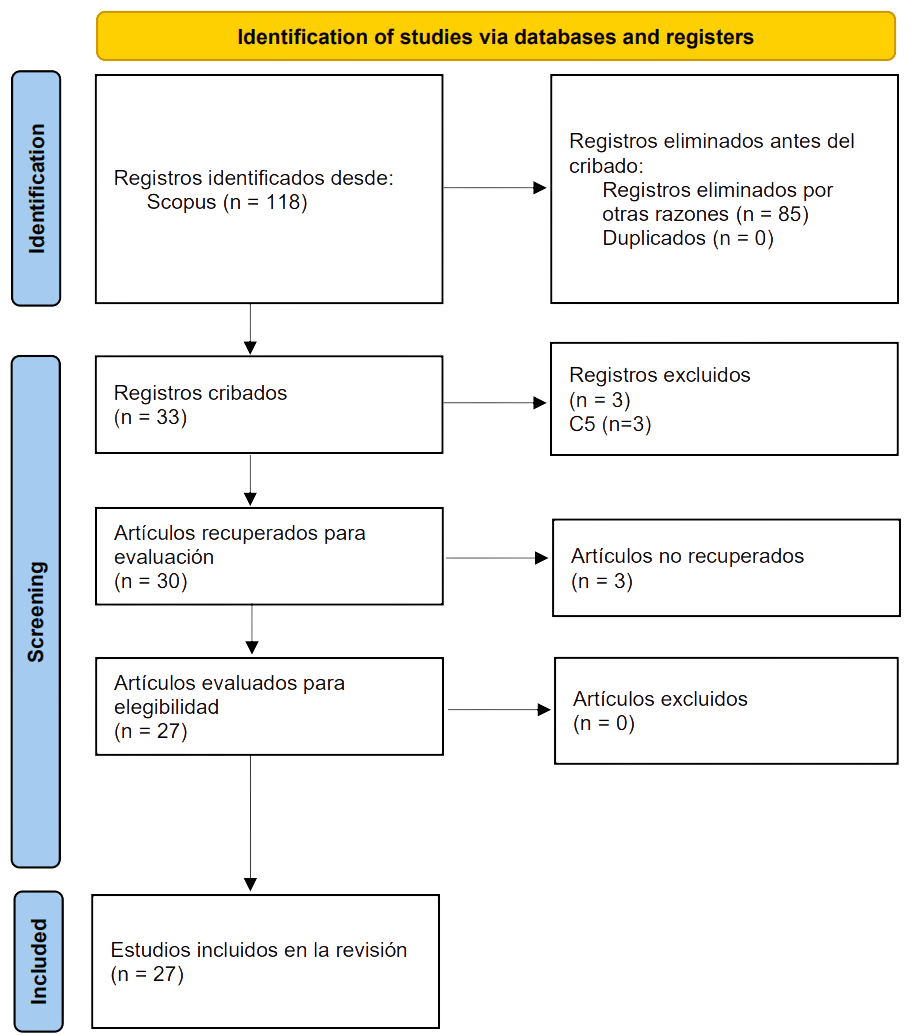
\includegraphics[width=7.8cm]{figures/fig1.png}
\end{center}
\caption{Diagrama de Prisma}
\label{figura1}
\end{figure}


\section{Resultados y Discusión}

Los resultados han sido divididos en dos partes: bibliométricos e ingeniería. 

\subsection{Resultados bibliometricos}
Luego del proceso de identificación de documentos científicos especificado en la figura 1, los artículos fueron ordenados según su año de publicación. En la figura 2, se puede identificar cómo en los últimos años el 2025 tuvo la mayor cantidad de producción científica con 10 artículos publicados, lo cual a su vez representa el 37\% con respecto al total.

\begin{figure}[H]
\begin{center}
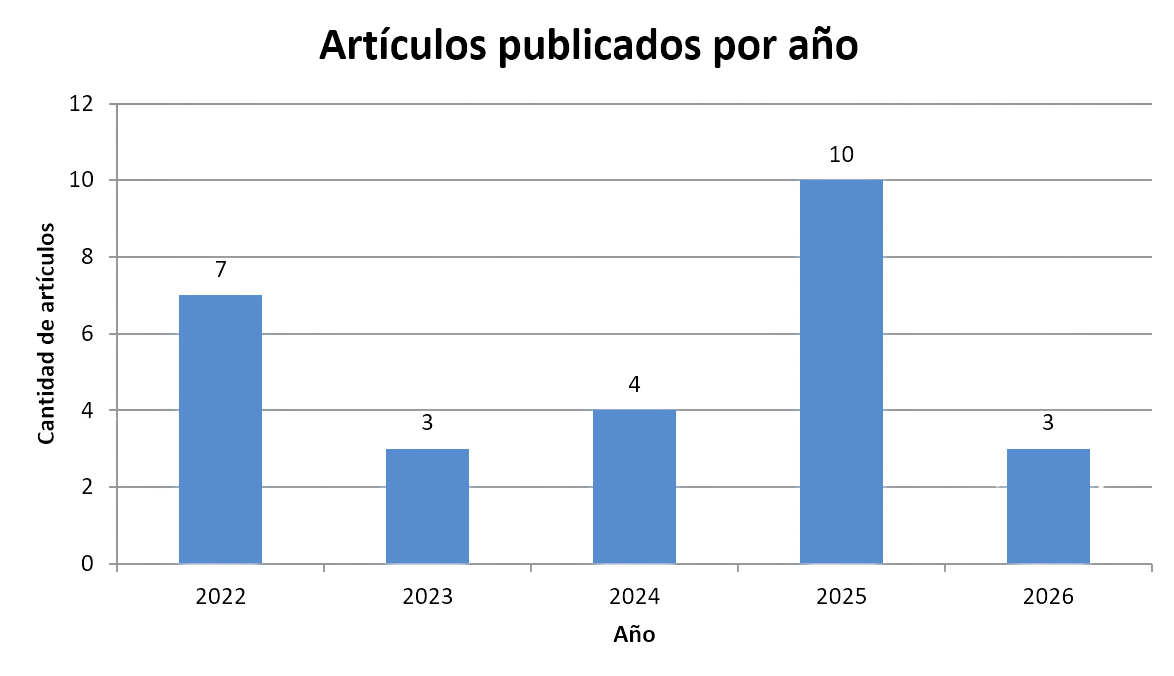
\includegraphics[width=8cm]{figures/fig3.png}
\end{center}
\caption{Artículos científicos por año}
\label{figura3}
\end{figure}


\begin{figure}[H]
\begin{center}
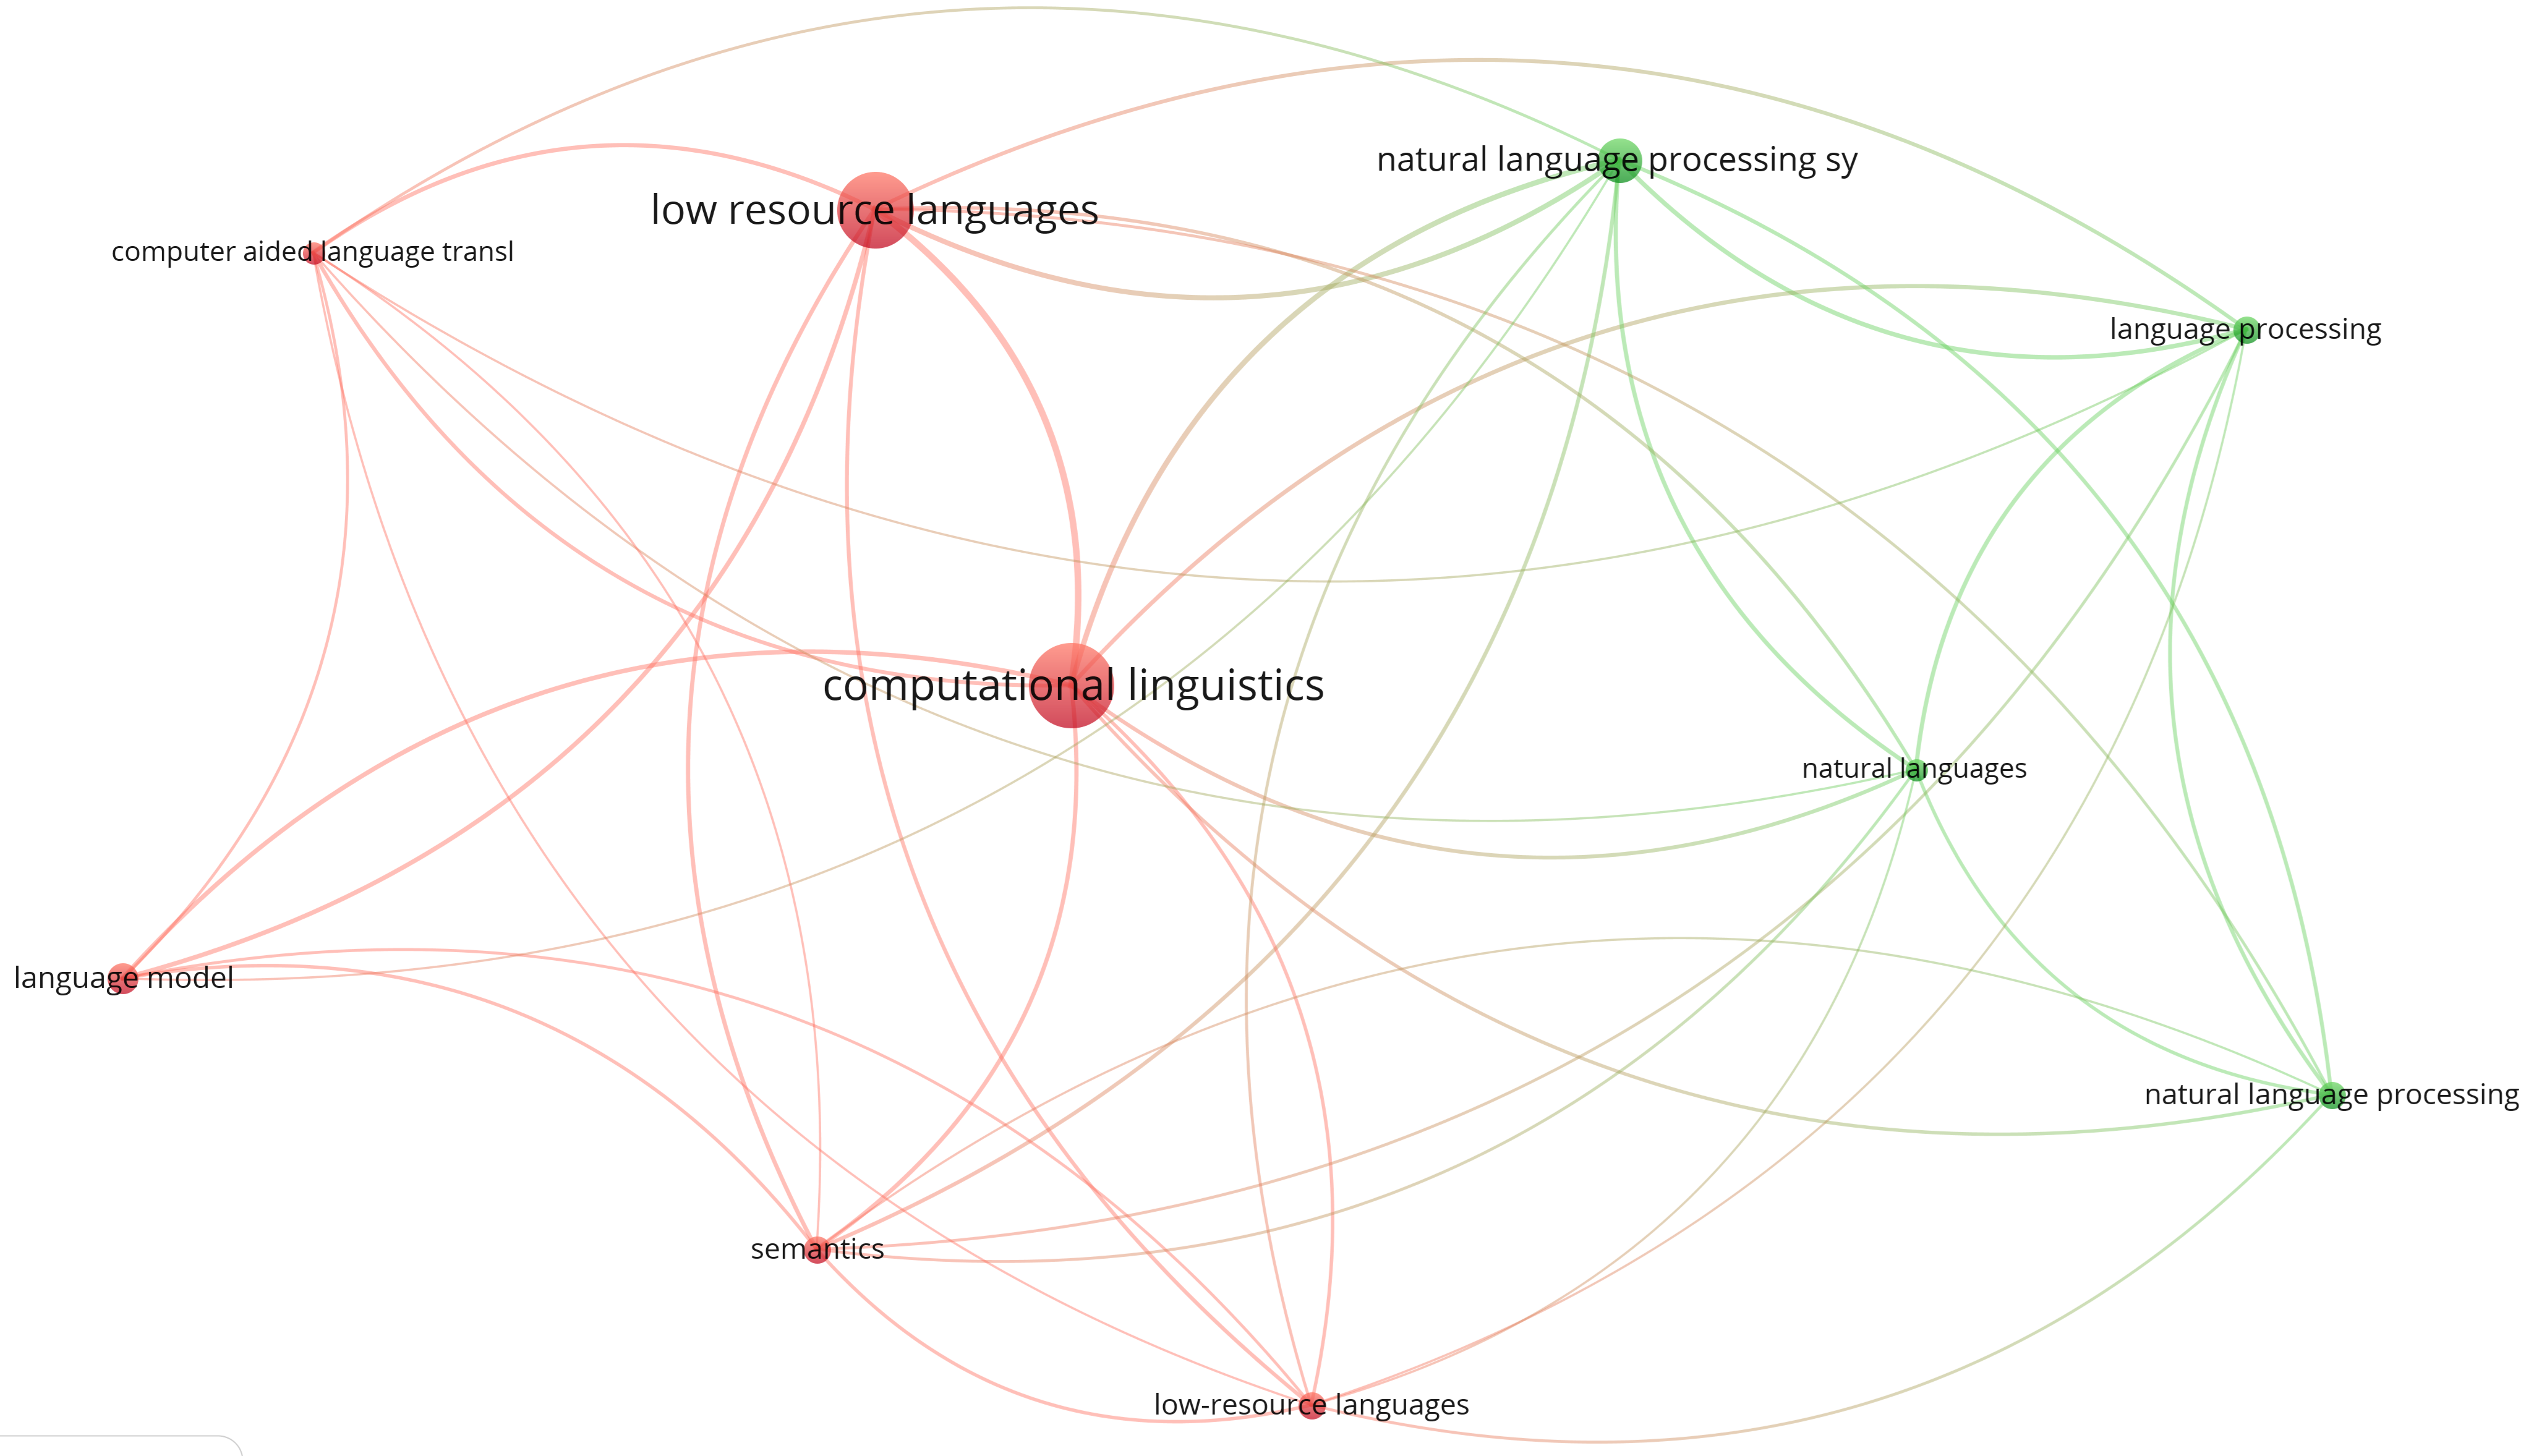
\includegraphics[width=8cm]{figures/fig4.png}
\end{center}
\caption{Red de coocurrencia de palabras clave}
\label{figura4}
\end{figure}

La figura 3 presenta la red de coocurrencia, la cual evidencia cómo se relacionan las palabras clave dentro de los artículos analizados. Se estableció un umbral de un mínimo de 5 ocurrencias por término, de las cuales solo 10 de 256 cumplieron este criterio. Asimismo, los conceptos con mayor centralidad son \textit{computational linguistics} con 19 ocurrencias, y \textit{low resource languages} con 17 ocurrencias; la proximidad entre ambos nodos y la mayor densidad de enlace, reflejan la alta frecuencia de aparición conjunta de ambas palabras clave. Por otro lado, es posible identificar por los colores rojo y verde la división entre dos grupos: el primero (rojo), agrupa las palabras orientadas a modelos, semántica y lenguajes de bajos recursos; mientras que el segundo (verde), destaca por su relación con el Procesamiento de Lenguaje Natural (NLP).

\begin{figure}[H]
\begin{center}

\includegraphics[width=8cm]{figures/fig8.png}
\end{center}
\caption{Distribuición geográfica de los artículos}
\label{figura5}
\end{figure}

La figura 4 muestra la distribuición geográfica de los estudios según el país de afiliación de los autores. Se observa que la producción científica está liderada por Estados Unidos con 6 artículos, lo cual representa el 22\% del total de la muestra. A este le siguen China e India, con una contribución de 3 artículos cada uno (11\% respectivamente), mientras que Arabia Saudita y Nueva Zelante con 2 publicaciones por nación. 
Asimismo, se destaca que la categoría otros países concentra el mayor volumen con 10 artículos, equivalente al 37\% del total, aportando cada país una sola producción. Esta categoría está integrada por Brasil, Canadá, Ecuador, España, Corea del Sur, México, Taiwán, Marruecos, Australia y Alemania. Finalmente, un solo estudio se clasificó como no especificado debido a la ausencia de datos explícitos sobre la procedencia de los autores.

A partir de estos resultados, se evidencia que, aun cuando la mayoría de producción científica recae en potencias tecnológicas como Estados Unidos y China, existe una gran descentralización geográfica.

\begin{figure}[H]
\begin{center}
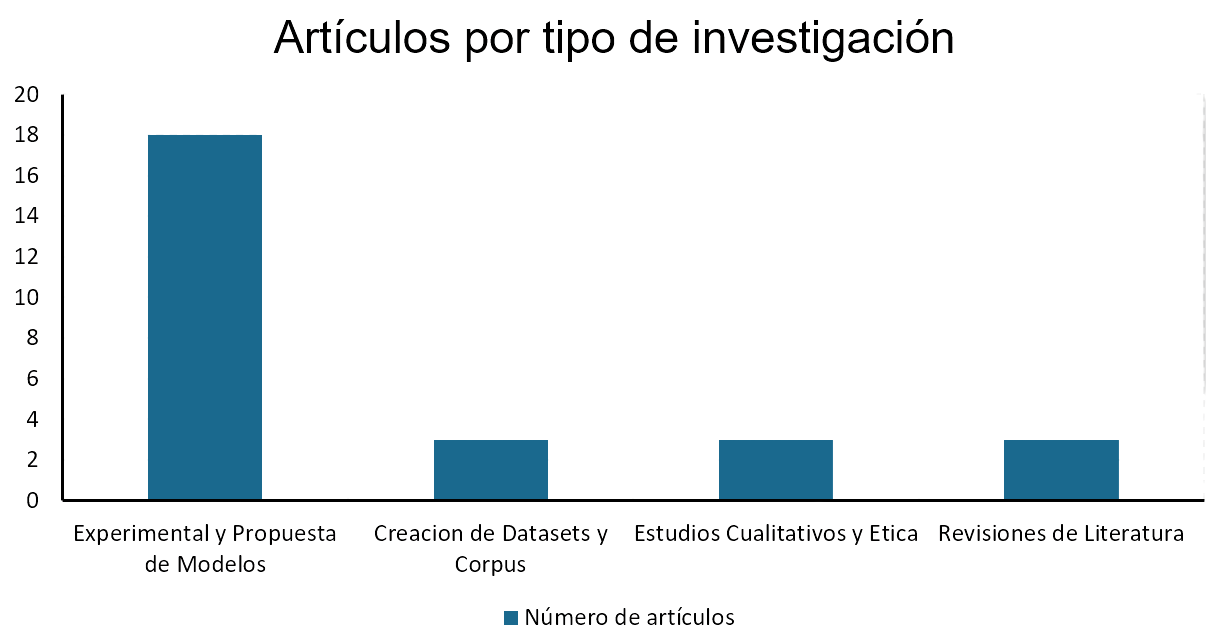
\includegraphics[width=8cm]{figures/fig9.png}
\end{center}
\caption{Tipo de investigación de los artículos}
\label{figura6}
\end{figure}

La figura 5 presenta la clasificación metodológica de los artículos, se observa un predominio de la investigación experimental y propuesta de modelos, la cual engloba 18 artículos científicos y representa el 66.7\% del total. Por otro lado, el tercio restante de las investigaciones se distribuye de manera uniforme con 3 artículos (11.1\%) por categoría: creación de bases de datos (datasets) y corpus, estudios cualitativos, sociales y de ética, y revisiones de la literatura. En base a esta información, se evidencia que la tendencia principal de la investigación actual se concentra principalmente en el diseño, entrenamiento y evaluación de arquitecturas algorítmicas, como modelos Transformer o de redes neuronales; en contraste, los estudios dedicados a la construcción de recursos lingüísticos, evaluación del impacto humano y estado del arte, representan, hasta el momento, una minoría.


\subsection{Resultados de ingeniería}
La recopilación de la información se realizó tomando principalmente las preguntas PICO formuladas. 

P: ¿De qué manera las tecnologías de Procesamiento de Lenguaje Natural (NLP) benefician la integración de la lengua materna en entornos educativos?

Las tecnologías de NLP aportan positivamente en la integración de la lengua materna en entornos educativos al facilitar el desarrollo de herramientas de aprendizaje que ayudan con las limitaciones de la enseñanza tradicional como la marginación lingüística y falta de materiales debido a que las instituciones tienden a priorizar idiomas de alta difusión \cite{Wakhare2026}. Por ejemplo, la aplicación móvil Wawa fue desarrollada como una herramienta educativa para el aprendizaje de la lengua kichwa, al evaluarla en estudiantes de las comunidades del río Napo en Loreto (Perú) los resultados indicaron que Wawa es una herramienta efectiva para aprender Kichwa sobrepasando la enseñanza tradicional \cite{Vallejo-Huanga2026}. 

Asimismo, ATAIGI, que significa "aprender hokkien taiwanés", es una aplicación de aprendizaje del idioma hokkien taiwanés el cual combina varios modelos generativos: \textit{Taiwanese Hokkien Translation Model introduced} para traducir mandarín e inglés desde y hacia hokkien taiwanés; \textit{fine-tunning} con un modelo supervisado pre-entrenado \textit{Hokkien 13B}; \textit{DALL-E 3} de OpenAI API para texto a imagen; y \textit{Hokkien transliteration movel}. El estudio demuestra cerrar brechas comunicacionales e incrementar la competencia lingüística, se evaluó la aplicación en 25 participantes de los cuales tras un mes de uso semanal se registró un incremento medio de 18 puntos en las pruebas de competencia lingüística, además que el modelo llegó a superar los resultados medidos sobre GPT-4 y otros modelos base de \textit{LLaMA} \cite{Chu2025}. 
Estas integraciones tecnológicas motivan a los estudiantes a vincular lo nuevo aprendido directamente con sus experiencias previas, apoyando el desarrollo cognitivo, razonamiento moral y la formación de su identidad social comunitaria \cite{Wakhare2026}.

Con el fin de organizar la información, la tabla 3 sintetiza los hallazgos previamente mencionados.

\begin{table}[H]
\centering
\captionof{table}{Aplicaciones de NLP para la integración de lenguas maternas en entornos educativos}
\small
    \begin{tabular}{p{2.2cm}p{4.8cm}}
    \toprule
    \multicolumn{2}{c}{\textbf{Wawa}} \\
    \midrule
    \textbf{Lengua} & Kichwa \\ \addlinespace
    \textbf{Enfoque NLP} & Aplicación móvil educativa para el aprendizaje de lengua materna. \\ \addlinespace
    \textbf{Aporte educativo} & Favorece el aprendizaje del kichwa en estudiantes de comunidades del río Napo. \\
    \midrule
    \multicolumn{2}{c}{\textbf{ATAIGI}} \\
    \midrule
    \textbf{Lengua} & Hokkien taiwanés \\ \addlinespace
    \textbf{Enfoque NLP} & Traducción automática, fine-tuning de modelo Hokkien 13B, generación texto-imagen con DALL-E 3 y transliteración. \\ \addlinespace
    \textbf{Aporte educativo} & Incremento medio de 18 puntos en competencia lingüística tras un mes de uso semanal en 25 participantes. \\
    \bottomrule
    \end{tabular}
\label{tab:nlp_lengua_materna_educacion}
\end{table}


I: ¿De qué manera las herramientas basadas en Inteligencia Artificial (IA) y los Grandes Modelos de Lenguaje LLMs mejoran la accesibilidad educativa?
Las herramientas basadas en IA y  LLMs mejoran la accesibilidad educativa al disminuir de manera efectiva las barreras lingüísticas. Por ejemplo, el desarrollo de aplicaciones multimodales basados en modelos generativos permite crear entornos de aprendizaje interactivos \cite{Chu2025}. Del mismo modo, la incorporación de reconocimiento de voz ayuda a entrenar la pronunciación oral \cite{Akallouch2025}.

La figura 6 muestra los diferentes tipos de área de implementación NLP que abarcaron las investigaciones, es posible observar que la mayoría se concentra en herramientas de traducción automática, seguida por reconocimiento automático de voz y la segmentación morfológica. Para hacer frente a la escasez de corpus paralelos se usó descripciones lingüísticas y diccionarios mediante \textit{in-context learning} logrando una alta eficacia incluso en áreas de razonamiento matemático \cite{Zhang2024}. Asimismo, la integración de redes neuronales con técnicas de meta-aprendizaje como \textit{Model-Agnostic Meta-Learning} (MAML) permite traducciones y transcripciones en tiempo real \cite{Fakhreldin2025}. 


\begin{figure}[H]
\begin{center}
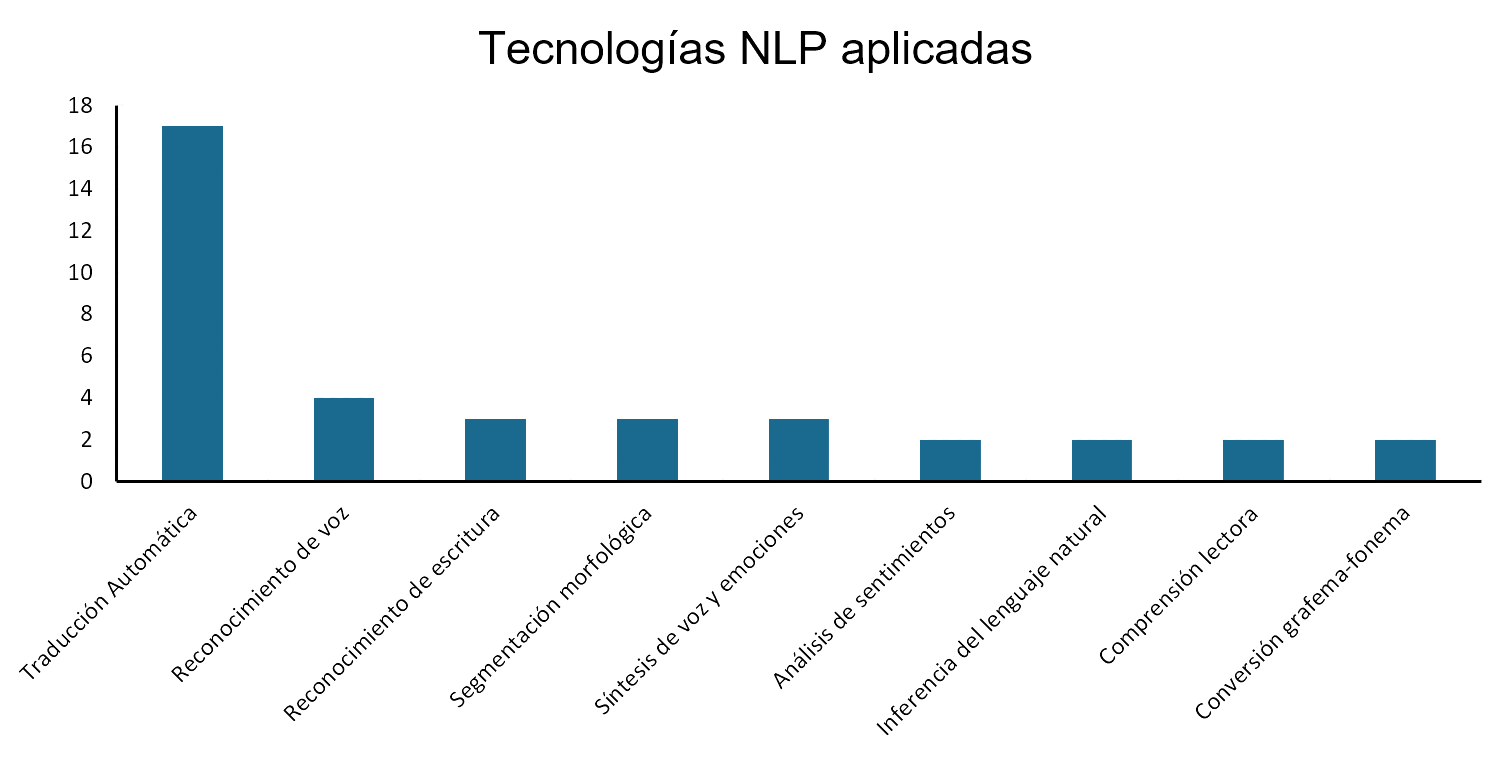
\includegraphics[width=8cm]{figures/fig10.png}
\end{center}
\caption{Aplicaciones NLP}
\label{figura6}
\end{figure}


C: ¿Qué vacíos existen entre el desempeño de la IA en lenguas de alto recurso frente a las de bajos recursos?
Existen brechas significativas en el desempeño de herramientas basadas en IA entre lenguas de alto recurso y lenguas de bajos recursos. Por ejemplo, en tareas de comprensión semántica, en \cite{Ebrahimi2022} se evaluó el modelo multilingüe \textit{Cross-Lingual Language Modeling-Roberta}(XLM-R) en un escenario \textit{zero-shot} sobre 10 lenguas indígenas, obteniendo una precisión promedio de solo 38.48\%. De manera similar, en \cite{Zhang2024} se observó que, bajo en enfoques \textit{zero-shot}, los LLMs obtienen valores de \textit{BiLingual Evaluation Understudy} (BLEU) menores a 1 en la mayoría de las 8 lenguas evaluadas. Por otro lado, estas brechas también se evidencian en aspectos relacionados con la seguridad y alineamiento de los LLMs, en \cite{Shen2024} se reportó que los modelos tienden a generar respuestas más dañinas cuando los \textit{prompts} están escritos en lenguas de bajos recursos, por ejemplo, en GPT-4, la tasa de respuestas dañinas fue de 35\% en comparación con 1\% en lenguas de alto recurso; asimismo, en el modelo Llama-2, la capacidad de seguimiento de instrucciones en lenguas de bajos recursos fue de 24.8\% en comparación al 33\% que se obtiene en lenguas de altos recursos. También, la escasez de corpus paralelos induce anomalías como la memorización (\textit{rogue memorization}) de respuestas exactas en vez de razonar, donde el modelo repite frases del entrenamiento en lugar de traducir \cite{Cavalin2024}.

En conclusión, las lenguas de bajo recursos no solo enfrentan limitaciones en cuanto a rendimiento, sino también problemas asociados a la seguridad y confiabilidad. A modo de síntesis, la tabla 3 resume las diferencias identificadas en los estudios revisados.

\begin{table}[H]
\centering
\captionof{table}{Comparación de desempeño de la IA entre lenguas de alto y bajo recurso}
\small
    \begin{tabular}{p{2.2cm}p{4.8cm}}
    \toprule
    \textbf{Métrica} & \textbf{Comparación} \\
    \midrule
    Comprensión semántica & XLM-R obtuvo una precisión promedio de 38.48\% en un escenario \textit{zero-shot} sobre 10 lenguas indígenas \cite{Ebrahimi2022}. \\ \addlinespace

    Traducción automática & Los LLMs alcanzaron valores de BLEU menores a 1 en la mayoría de las 8 lenguas evaluadas \cite{Zhang2024}. \\ \addlinespace

    Seguridad y alineamiento & GPT-4 presentó una tasa de respuestas dañinas de 35\% en lenguas de bajos recursos, frente a 1\% en lenguas de alto recurso \cite{Shen2024}. \\ \addlinespace

    Seguimiento de instrucciones & Llama-2 alcanzó 24.8\% de seguimiento de instrucciones en lenguas de bajos recursos, frente a 33\% en lenguas de alto recurso \cite{Shen2024}. \\ \addlinespace

    Confiabilidad del modelo & La escasez de corpus paralelos puede inducir \textit{rogue memorization} \cite{Cavalin2024}. \\
    \bottomrule
    \end{tabular}
\label{tab:brechas_ia_lenguas}
\end{table}


O: ¿Qué estrategias y metodologías son las más eficaces para mejorar la accesibilidad educativa?
Las estrategias y metodologías más eficaces para mejorar la accesibilidad educativa son las que mitigan directamente las limitaciones que enfrentan las lenguas de bajos recursos para el desarrollo de herramientas efectivas, entre ellas se identificó a las que combinan herramientas algorítmicas como el uso de meta-aprendizaje (MAML) \cite{Fakhreldin2025}, implementación de arquitecturas híbridas \cite{Chang2025}, inyección de conocimiento lingüístico \cite{Zhang2024}; y aquellas que tienen un enfoque participativo con la población de estudio como en \cite{Liu2022} donde se consulta directamente con maestros y hablantes nativos, o en \cite{Mager2023} que garantizan la soberanía de los datos a las comunidades indígenas garantizando de esta manera evitar la distorsión del conocimiento \cite{Rathnayake2026}.

\begin{figure}[H]
\begin{center}
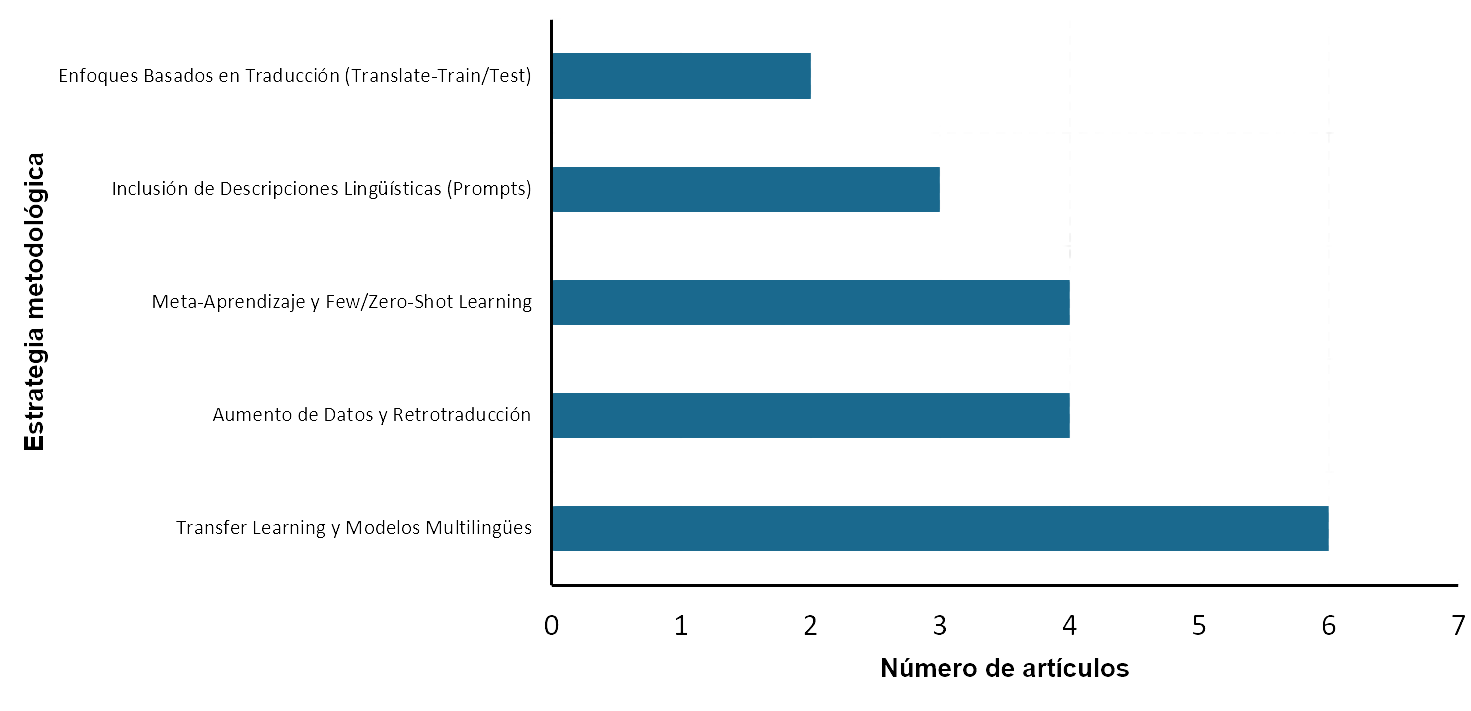
\includegraphics[width=8cm]{figures/fig7.png}
\end{center}
\caption{Estrategias para Mitigar la Escasez de Datos}
\label{figura7}
\end{figure}

La figura 7 muestra como el \textit{transfer learning}, modelos multilingües y el aumento de datos son los enfoques técnicos más frecuentes para mitigar la escasez de datos, en \cite{Liu2022} \cite{Chang2025} se evidencia que la falta de corpus digitalizados representa una de las barreras principales que impide el desarrollo eficaz de tecnologías de NLP.


\subsection{Discusión}
En general, la literatura científica actual acerca de las aplicaciones y usos de la inteligencial artificial en lenguas de bajos recursos lingüisticos es alentador porque se puede evidenciar que se le está dando más importancia al tema de investigación, hay esperanzas en evitar lo que en \cite{Zhang2024}, \cite{Cavalin2024} se menciona: que en las próximas décadas las lenguas de bajo recursos desaparezcan. La cantidad de artículos científicos incrementó del año 2024 al 2025, siendo la mayoría propuestas de modelos (66.7\%), de los cuales la mayoría son de traducción automática. Al respecto, se llega a comprobar que arquitecturas estándar o de LLMs evaluados en escenarios \textit{zero-shot} obtienen métricas BLEU cercanas a cero debido a la ausencia de estas lenguas durante su preentrenamiento; además, realizar \textit{fine-tunning} habiendo escacez extrema de datos puede inducir anomalías como la memorización descontrolada (\textit{rogue memorization}). No obstante, se logró demostrar mediante diferentes enfoques diseñados para mitigar la escacez de datos que se pueden superar estos obstáculos: se logró pasar en la escala BLEU de 0 a un promedio de 10.5 usando descripciones gramaticales y diccionarios mediante el aprendizaje en contexto (\textit{in-context learning}) \cite{Zhang2024}; para compensar la escacez de datos integraron traducción automática neuronal (NMT) con traducción basada en frases (PBMT) \cite{Chang2025}; en la traducción de la lengua maorí a inglés \cite{Gao2026}, se implementó representaciones contextualizadas de oraciones incrementando hasta 1.46 puntos en la escala BLEU; el modelo XLM-SWCM (\textit{Cross-lingual Language Model with Shared Weights Cross-lingual Modeling}) superó el modelo mBART (\textit{Multilingual BART}) en un 199\% en resumen de textos y 108\% en comprensión de lectura \cite{Su2025}. 

A su vez, es importante recalcar que los estudios evaluados señalan varias limitaciones que aún deben de superarse, como lo es la dependencia a métricas para evaluar el rendimiento de la traducción automática como BLEU (\textit{Bilingual Evaluation Understudy}), TER (\textit{Translation Error Rate}) o WER (\textit{Word Error Rate}), ya que no se llega a capturar adecuadamente matices culturales y el significado contextual en lenguas de bajos recursos \cite{Park2025}, y en el caso de reconocimiento de voz, no se llega a diferenciar entre variantes morfológicas, diferencias dialectales y patrones de orden de palabras flexible \cite{Akallouch2025}. 
Asimismo, muchos de los modelos propuestos se limitan a una sola  variante dialectual de la lengua estudiada, por lo que las demás variantes quedan sin evaluar \cite{Park2025, Santiago-Benito2025, Akallouch2025}. Las lenguas minoritarias suelen carecer de ortografía estandarizada y poseer complejidad morfofonémica lo cual dificulta el procesamiento del texto, ya que los modelos pueden fallar al segmentar palabras, reconocer raíces y morfemas \cite{Liu2022, Manimaran2024, Vallejo-Huanga2026, Akallouch2025}.

En este contexto, para superar las limitaciones actuales y mejorar los resultados obtenidos, se sugiere a las futuras investigaciones adoptar un enfoque participativo con los hablantes de las lenguas estudiadas y priorizar sus necesidades con el fin de desarrollar herramientas útiles para su uso. No hay que olvidar que el propósito de desarrollar aplicaciones o tecnologías nuevas es para resolver un problema específico, una necesidad o facilitar una tarea, y para muchas de estas lenguas sus prioridades son documentar, enseñar y reavivar su lengua, preservar su identidad, patrimonio transmitido por generaciones y hacer que su lengua tenga voz frente a otros idiomas. Por otro lado, también se recomienda evitar la dependencia excesiva a textos religiosos como la biblia ya que puede inducir \textit{rogue memorization}, y en su lugar recopilar y construir un corpus que abarce diferentes áreas. Finalmente, resulta de vital importancia abordar la diversidad dialectal y evitar entrenar modelos que estandaricen una lengua en base a solo una variante o dialecto.


%========================================================
\section{Conclusiones}

Esta revisión tuvo como objetivo sintetizar los enfoques metodológicos empleados, resultados educativos reportados e identificar los principales desafíos y oportunidades. Los hallazgos evidencian que la inteligencia artificial aplicada a lenguas de bajos recursos se encuentra en crecimiento, aunque todavía presenta una producción científica limitada y dispersa. No obstante, se identificó un incremento en las publicaciones del año 2024 al 2025. Asimismo, la mayor parte de las publicaciones corresponde a investigaciones experimentales y propuestas de modelos las cuales representan el 66.7\% del total de la muestra. 

En cuanto a aplicaciones educativas, los resultados muestran que aplicaciones basadas en NLP contribuyen positivamente a integrar la lengua materna en entornos de aprendizaje con resultados más satisfactorios que los de una enseñanza tradicional. Por otro lado, entre las estrategias más utilizadas para enfrentar la falta de corpus y mejorar el desempeño de los modelos, se identifica el uso de descripciones lingüísticas, diccionarios mediante \textit{in-context learning} y técnicas de meta-aprendizaje. A su vez, otro hallazgo relevante es la existencia de brechas significativas en cuanto al rendimiento de herramientas basadas en IA entre lenguas de alto recurso y lenguas de bajos recursos, se reportaron distintas limitantes en tareas de comprensión semántica, traducción automática, seguimiento de instrucciones, seguridad y confiabilidad de los modelos.
En relación con las estrategias metodológicas, se evidenció que los enfoques más destacables combinan técnicas algorítmicas con metodologías participativas, como el \textit{transfer learning}, modelos multilingües, aumento de datos, meta-aprendizaje, arquitecturas híbridas y la inyección de conocimiento lingüístico. Sin embargo, también se resalta la importancia de involucrar a la población de estudio en el diseño y evaluación de las herramientas a fin de evitar la distorsión del conocimiento, respetar la soberanía sobre los datos y asegurar que las soluciones respondan a sus necesidades.
Finalmente, esta revisión sistemática de la literatura identifica desafíos que deben ser abordados en futuras investigaciones, entre ellas se encuentran la escasez de corpus digitalizados, dependencia excesiva de métricas como BLEU, TER o WER, la falta de inclusión de más de una variante dialectal, ausencia de ortografías estandarizadas y la complejidad morfofonémica. Aunque la inteligencia artificial representa una vía prometedora para mejorar la accesibilidad educativa en lenguas de bajos recursos, su implementación requiere enfoques más participativos que involucren a la población de estudio, prioricen sus necesidades y también tener en cuenta la variedad dialectal. La participación de hablantes nativos podría contribuir a crear mejores datos de entrenamiento y evitar errores culturales o de significado.
%========================================================

\section*{Agradecimientos}

El autor expresa su agradecimiento al profesor Jose Luis Briones Zuñiga por su orientación y acompañamiento brindado durante el desarrollo de este trabajo; a Yishar Piero Nieto Barrientos, por su apoyo y motivación 

Este apartado es opcional que dependerá su utilización en caso de exister algun organismo financiador, colaborador, etc., que permitió llevar a cabo la investigación.
%========================================================


\bibliography{referencias.bib}
\bibliographystyle{IEEEtran}
\end{multicols}
\end{document}